\section{Register description}
\regover{
{\hyperref[l1c-l1c-config]{l1c\_config}}&L1C configuration
\\
\hline
{\hyperref[l1c-hit-cnt-lsb]{hit\_cnt\_lsb}}&Low 32-bit hit couter
\\
\hline
{\hyperref[l1c-hit-cnt-msb]{hit\_cnt\_msb}}&High 32-bit hit counter
\\
\hline
{\hyperref[l1c-miss-cnt]{miss\_cnt}}&Miss counter
\\
\hline
}

\subsection{l1c\_config}
\label{l1c-l1c-config}
Address:0x40009000
 \begin{figure}[H]
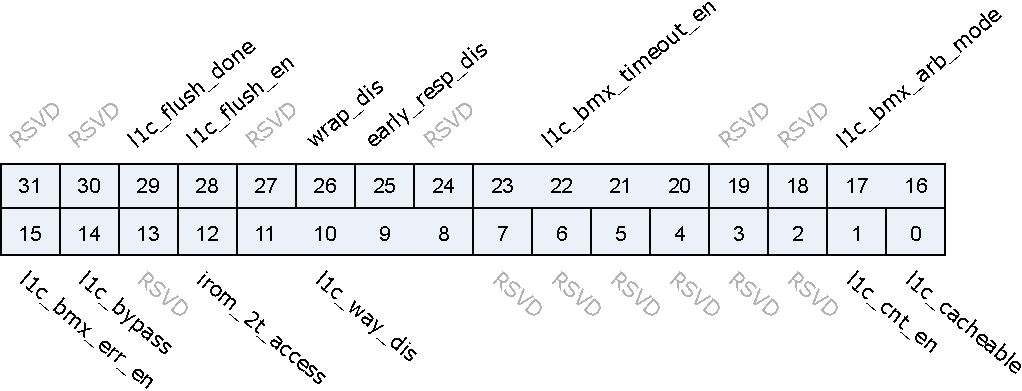
\includegraphics{l1c_l1c_config.pdf}
\end{figure}

\regdes{31:30&RSVD& & & \\\hline
29&l1c\_flush\_done&r&0&\\\hline
28&l1c\_flush\_en&r/w&0&flush dirty line\\\hline
27&RSVD& & & \\\hline
26&wrap\_dis&r/w&1&\\\hline
25&early\_resp\_dis&r/w&1&\\\hline
24&RSVD& & & \\\hline
23:20&l1c\_bmx\_timeout\_en&r/w&0&Bus timeout enable: detect slave no reaponse in 1024 cycles\\\hline
19:18&RSVD& & & \\\hline
17:16&l1c\_bmx\_arb\_mode&r/w&0&[1:0] 0:fix, 2:round-robin, 3:random\\\hline
15&l1c\_bmx\_err\_en&r/w&0&Bus error response enable\\\hline
14&l1c\_bypass&r/w&0&bypass cache ; reset cache\\\hline
13&RSVD& & & \\\hline
12&irom\_2t\_access&r/w&0&Set 1 for ROM 2T access if CPU freq >72MHz\\\hline
11:8&l1c\_way\_dis&r/w&4'b1111&Disable part of cache ways \& used as ITCM\\\hline
7:2&RSVD& & & \\\hline
1&l1c\_cnt\_en&r/w&0&\\\hline
0&l1c\_cacheable&r/w&0&\\\hline

}
\subsection{hit\_cnt\_lsb}
\label{l1c-hit-cnt-lsb}
Address:0x40009004
 \begin{figure}[H]
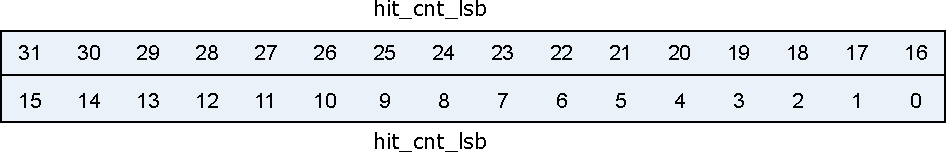
\includegraphics{l1c_hit_cnt_lsb.pdf}
\end{figure}

\regdes{31:0&hit\_cnt\_lsb&r&0&\\\hline

}
\subsection{hit\_cnt\_msb}
\label{l1c-hit-cnt-msb}
Address:0x40009008
 \begin{figure}[H]
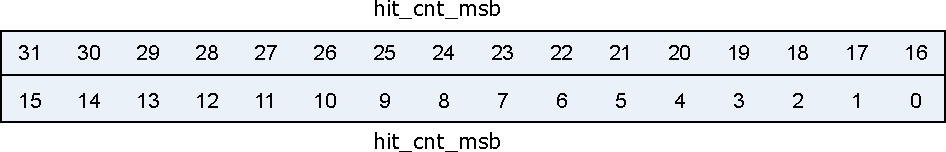
\includegraphics{l1c_hit_cnt_msb.pdf}
\end{figure}

\regdes{31:0&hit\_cnt\_msb&r&0&total hit count = hit\_cnt\_msb*2\^32 + hit\_cnt\_lsb\\\hline

}
\subsection{miss\_cnt}
\label{l1c-miss-cnt}
Address:0x4000900c
 \begin{figure}[H]
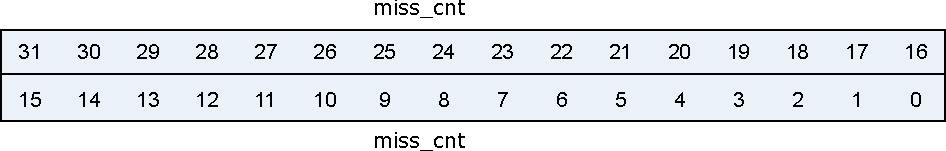
\includegraphics{l1c_miss_cnt.pdf}
\end{figure}

\regdes{31:0&miss\_cnt&r&0&\\\hline

}
